
\providecommand{\Cat}{\mathcal{C}at}
\providecommand{\sSet}{s\mathcal{S}et}
\providecommand{\wlim}{\operatorname{lim}}
\providecommand{\wcolim}{\operatorname{colim}}
\providecommand{\lan}{\operatorname{lan}}
\providecommand{\ran}{\operatorname{ran}}
\providecommand{\Fun}{\operatorname{Fun}}
\providecommand{\qcor}[1]{\ulcorner#1\urcorner}   %

\section{\trWeightedLimit{}与\trWeightedColimit}\label{sec:weighted-limits-and-colimits}

A.4 节的余张量与 A.5 节的锥形极限，皆为我们如今引入的更为一般的%
\emph{\trWeightedLimit}概念的实例。我们继续在\trComplete{}且\trCocomplete{}的%
\trCartesianClosed{}\trCategory{} $(\mathcal{V},\times,1)$ 的语境中工作。我们
心目中的例子是 $(\sSet,\times,1)$、其\trCartesianClosed{}子范畴
$(\Cat,\times,1)$，或者再往下一层的\trCartesianClosed{}子范畴
$(\mathcal{S}et,\times,1)$。

通常的\trLimit{}与\trColimit{}是那样一些对象：它们表示「以一个给定峰顶居于
一个固定\trDiagram{}之上或居于其下」的诸锥所构成的\trFunctor。\trWeightedLimit%
{}与\trWeightedColimit{}以类似的方式定义，不同之处只在于：居于一个\trDiagram%
{}之上或之下的诸锥可以带有\trExotic{}「形状」，而且这些形状容许随加标于该%
\trDiagram{}的那些对象而变化。更正式地，在 $\mathcal{V}$-富集的语境中，%
\emph{权}（weight）——它定义居于一个由 $\mathcal{A}$ 加标的\trDiagram{}之上、
或居于一个由 $\mathcal{A}^{\mathrm{op}}$ 加标的\trDiagram{}之下的锥之「形状」
——取 $\mathcal{V}^{\mathcal{A}}$ 中一个\trFunctor{}的形式；注意加标范畴
$\mathcal{A}$ 可以是 $\mathcal{V}$-富集的，这与 A.5 节所考虑的诸\trDiagram%
{}不同。

我们将从三种不同的视角发展\trWeightedLimit{}与\trWeightedColimit{}的一般概念，
并按与逻辑顺序相反的次序引入这三者，因为我们发现这条路线最为直观。我们首先
描述——当它们存在时——刻画\trWeightedLimit{}与\trWeightedColimit{}二函子的
那些公理。继而解释：在假定某些其他\trLimit{}与\trColimit{}存在的条件下，
\trWeightedLimit{}与\trWeightedColimit{}可以如何被构造出来。最后我们引入定义
一个特定的\trWeightedLimit{}或\trWeightedColimit{}的一般\trUniversalProperty，
它确切地规定了刚刚引入的那些概念要真正存在所需的一切。

\begin{definition}[\trWeightedLimit{}与余极限，公理式的]\label{def:weighted-limit-colimit-axiomatic}
对一个小的 $\mathcal{V}$-范畴 $\mathcal{A}$ 与一个大的 $\mathcal{V}$-范畴
$\mathcal{C}$，\textbf{\trWeightedLimit}与\textbf{\trWeightedColimit{}二函子}
\[ \wlim_{-}\colon(\mathcal{V}^{\mathcal{A}})^{\mathrm{op}}\times
     \mathcal{C}^{\mathcal{A}}\to\mathcal{C}
   \qquad\text{以及}\qquad
   \wcolim_{--}\colon\mathcal{V}^{\mathcal{A}}\times
     \mathcal{C}^{\mathcal{A}^{\mathrm{op}}}\to\mathcal{C} \]
在它们存在之时，由下述一对公理刻画：
\begin{itemize}
\item 带可表示之权的加权余／极限在表示对象处求值：
\[ \wlim_{\mathcal{A}(a,-)}F\cong Fa
   \qquad\text{以及}\qquad
   \wcolim_{\mathcal{A}(-,a)}G\cong Ga. \]
\item 加权余／极限二函子在权上是余连续的：对任何\trDiagram{}
  $F\in\mathcal{C}^{\mathcal{A}}$ 与 $G\in\mathcal{C}^{\mathcal{A}^{\mathrm{op}}}$，
  \trFunctor{} $\wcolim_{-}G$ 保持\trColimit，而\trFunctor{} $\wlim_{-}F$ 把%
  \trColimit{}带为\trLimit。\footnote{更精确地说，正如%
  \cref{prop:weighted-limit-definitions-agree}所证明的，\trWeightedColimit%
  {}\trFunctor{} $\wcolim_{-}G$ 保持\trWeightedColimit，而%
  \trWeightedLimit{}\trFunctor{}
  $\wlim_{-}F$ 把\trWeightedColimit{}带为\trWeightedLimit。}
\end{itemize}
\end{definition}

我们把公理 (ii) 诠释为：权可以「按需定制」（made-to-order）——一个作为诸%
可表示\trFunctor{}的\trColimit{}而构造出的权——一切取值于 $\mathcal{V}$ 中的%
\trFunctor{}皆属此类——将会规定所期望的\trUniversalProperty。

\begin{definition}[\trWeightedLimit{}与余极限，构造式的]\label{def:weighted-limit-colimit-constructive}
以 $W\in\mathcal{V}^{\mathcal{A}}$ \textbf{加权}（weighted by）的\trDiagram{}
$F\in\mathcal{C}^{\mathcal{A}}$ 之\textbf{\trLimit}由函子余张量积（functor
cotensor product）计算：
\begin{rveq}\label{eq:functor-cotensor-product}
\wlim_{W}F\coloneqq\int\limits_{a\in\mathcal{A}}Fa^{Wa}
  \coloneqq\mathrm{eq}\left(\;
    \prod_{a\in\mathcal{A}}Fa^{Wa}
    \Longrightarrow
    \prod_{a,b\in\mathcal{A}}Fb^{\mathcal{A}(a,b)\times Wa}\;\right),
\end{rveq}
其中的乘积与等化子应按 A.5 节中的\cref{def:conical-limit-colimit}之意义诠释为锥形极限。等化子%
图表中的诸映射由 hom-对象 $\mathcal{A}(a,b)$ 在 $\mathcal{V}$-函子 $W$ 与 $F$
上的作用 $\mathcal{A}(a,b)\times Wa\to Wb$ 与 $Fa\to Fb^{\mathcal{A}(a,b)}$
诱导而出。
对偶地，以 $W\in\mathcal{V}^{\mathcal{A}}$ 加权的\trDiagram{}
$G\in\mathcal{C}^{\mathcal{A}^{\mathrm{op}}}$ 之\textbf{\trColimit}由函子张量积
（functor tensor product）计算：
\begin{rveq}\label{eq:functor-tensor-product}
\wcolim_{W}G\coloneqq\int\limits^{a\in\mathcal{A}}Wa\otimes Ga
  \coloneqq\mathrm{coeq}\left(\;
    \coprod_{a,b\in\mathcal{A}}\bigl(Wa\times\mathcal{A}(a,b)\bigr)\otimes Gb
    \Longrightarrow
    \coprod_{a\in\mathcal{A}}Wa\otimes Ga\;\right),
\end{rveq}
其中的余积与余等化子应诠释为锥形余极限。余等化子图表中的两支映射，一支由
$\mathcal{A}(a,b)$ 在反变 $\mathcal{V}$-函子 $G$ 上的作用
$\mathcal{A}(a,b)\otimes Gb\to Ga$ 诱导而出，另一支则一如前述地使用
$\mathcal{A}(a,b)$ 在 $W$ 上的协变作用。
\end{definition}

\begin{definition}[\trWeightedLimit{}与余极限，泛性质]\label{def:weighted-limit-colimit-universal-property}
\trDiagram{} $F\in\mathcal{C}^{\mathcal{A}}$ 以 $W\in\mathcal{V}^{\mathcal{A}}$
加权的\textbf{\trLimit} $\wlim_{W}F$ 与\trDiagram{}
$G\in\mathcal{C}^{\mathcal{A}^{\mathrm{op}}}$ 以 $W\in\mathcal{V}^{\mathcal{A}}$
加权的\textbf{\trColimit} $\wcolim_{W}G$ 由下述\trUniversalProperty{}刻画：
\begin{rveq}\label{eq:weighted-universal-property}
\mathcal{C}\bigl(x,\wlim_{W}F\bigr)\cong\mathcal{V}^{\mathcal{A}}\bigl(W,\mathcal{C}(x,F)\bigr)
\qquad\text{以及}\qquad
\mathcal{C}\bigl(\wcolim_{W}G,x\bigr)\cong\mathcal{V}^{\mathcal{A}}\bigl(W,\mathcal{C}(G,x)\bigr),
\end{rveq}
其中每一者都定义 $\mathcal{V}$ 中诸对象之间的一个\trIsomorphism，后者在 $x$ 上
是 $\mathcal{V}$-自然的。
\end{definition}

当加标范畴从上下文来看不明确时，我们可以在\trWeightedLimit{}与\trWeightedColimit{}的记号上添加
一个上标以指明它。\cref{prop:weighted-limit-definitions-agree}表明：这三个定义
刻画的是同样的对象。在证明它的途中，我们会得到一些因其自身之故而值得关切的
结果，并将它们单独记录如下。

\begin{lemma}\label{lem:complete-v-admits-weighted-limits}
一个\trComplete{}\trCartesianClosed{}\trCategory{} $\mathcal{V}$ 容有一切%
\trWeightedLimit——即由 \eqref{eq:functor-cotensor-product} 之公式所定义、满足
\eqref{eq:weighted-universal-property} 之自然\trIsomorphism{}与%
\cref{def:weighted-limit-colimit-axiomatic}之公理的\trWeightedLimit。显式地，对一个权
$W\colon\mathcal{A}\to\mathcal{V}$ 与一个\trDiagram{}
$F\colon\mathcal{A}\to\mathcal{V}$，\trWeightedLimit
\[ \wlim_{W}F\coloneqq\mathcal{V}^{\mathcal{A}}(W,F) \]
就是从 $W$ 到 $F$ 的诸 $\mathcal{V}$-\trNaturalTransformation{}的
$\mathcal{V}$-对象。\footnote{原书此处印作「from $W$ to $V$」；按上方显式公式
$\wlim_{W}F\coloneqq\mathcal{V}^{\mathcal{A}}(W,F)$，疑为「from $W$ to $F$」
之误，此处径改。——译者注}
\end{lemma}

\begin{proof}
由\trTerminal{}对象所表示的 $\mathcal{V}$-函子
$\mathcal{V}(1,-)\colon\mathcal{V}\to\mathcal{V}$ 自然同构于恒等\trFunctor。
于是，在\trDiagram{} $F\in\mathcal{V}^{\mathcal{A}}$ 取值于 $\mathcal{V}$-范畴
$\mathcal{V}$ 之中的情形下，于 \eqref{eq:weighted-universal-property} 的%
\trUniversalProperty{}中取 $x=1$，便有
\[ \wlim_{W}F\cong\mathcal{V}^{\mathcal{A}}(W,F). \]
与此同时，公式 \eqref{eq:functor-cotensor-product} 计算了%
\cref{def:vobject-natural-transformations}所引入的、从 $W$ 到 $F$ 的诸
$\mathcal{V}$-\trNaturalTransformation{}的 $\mathcal{V}$-对象
$\mathcal{V}^{\mathcal{A}}(W,F)$。\cref{thm:enriched-yoneda}的富集%
\trYonedaLemma{}证得第一条公理，而第二条公理可由
\eqref{eq:weighted-universal-property} 的\trUniversalProperty{}推出。
\end{proof}

诸 $\mathcal{V}$-\trNaturalTransformation{}的 $\mathcal{V}$-对象满足自然%
\trIsomorphism
\[ \mathcal{V}\bigl(v,\mathcal{V}^{\mathcal{A}}(W,F)\bigr)
   \cong\mathcal{V}^{\mathcal{A}}\bigl(W,\mathcal{V}(v,F)\bigr) \]
对任何 $v\in\mathcal{V}$。把「取值于 $\mathcal{V}$ 的诸\trFunctor{}的
$W$-\trWeightedLimit{}是诸\trNaturalTransformation{}的 $\mathcal{V}$-对象」这一观察应用
于诸\trFunctor{} $\mathcal{C}(x,F-)$ 与 $\mathcal{C}(G-,x)$，我们便可把自然%
\trIsomorphism{} \eqref{eq:weighted-universal-property} 重新表达为：

\begin{corollary}\label{cor:weighted-limits-representably-defined}
\eqref{eq:weighted-universal-property} 的\trWeightedLimit{}与\trWeightedColimit，作为 $\mathcal{V}$
中的\trWeightedLimit{}被可表示地定义：对 $W\in\mathcal{V}^{\mathcal{A}}$、
$F\in\mathcal{C}^{\mathcal{A}}$ 与 $G\in\mathcal{C}^{\mathcal{A}^{\mathrm{op}}}$，
\trWeightedLimit{}与\trWeightedColimit{}由在 $x$ 中 $\mathcal{V}$-自然的诸\trIsomorphism{}刻画：
\begin{rveq}\label{eq:weighted-representable-expression}
\mathcal{C}\bigl(x,\wlim_{W}F\bigr)\cong\wlim_{W}\mathcal{C}(x,F)
\qquad\text{以及}\qquad
\mathcal{C}\bigl(\wcolim_{W}G,x\bigr)\cong\wlim_{W}\mathcal{C}(G,x)
\end{rveq}
\end{corollary}

我们如今统一定义 A.6.1、定义 A.6.2 与定义 A.6.5 这三者。

\begin{proposition}\label{prop:weighted-limit-definitions-agree}
当 \eqref{eq:functor-cotensor-product} 与 \eqref{eq:functor-tensor-product} 的%
\trLimit{}与\trColimit{}存在时，它们所定义的对象满足\trUniversalProperty{}
\eqref{eq:weighted-universal-property}，或者等价地，满足
\eqref{eq:weighted-representable-expression}。由这些\trUniversalProperty{}所
定义的 $\mathcal{V}$-二函子满足\cref{def:weighted-limit-colimit-axiomatic}的
公理。
\end{proposition}

\begin{proof}
定义 A.6.2 与定义 A.6.5 之等价性——对\trWeightedLimit{}或\trWeightedColimit{}任一者而言——是
这一蕴含关系在取值于 $\mathcal{C}=\mathcal{V}$ 的\trWeightedLimit{}上的特例的直接推论，
后者已作为\cref{lem:complete-v-admits-weighted-limits}与%
\cref{cor:weighted-limits-representably-defined}证得。\eqref{eq:functor-cotensor-product}
中对 $\mathcal{A}$ 加标的诸\trLimit，同样以可表示的方式经由 $\mathcal{V}$ 中
类似的\trLimit{}来定义。于是，由 \eqref{eq:functor-cotensor-product} 所定义的
那个对象表示定义\trWeightedLimit{} $\wlim_{W}F$ 的 $\mathcal{V}$-\trFunctor{}
$\wlim_{W}\mathcal{C}(-,F)$。

尚须证明：定义 A.6.2 与定义 A.6.5 的\trWeightedLimit{}满足%
\cref{def:weighted-limit-colimit-axiomatic}的公理。在取值于 $\mathcal{V}$ 的%
\trDiagram{} $F\in\mathcal{V}^{\mathcal{A}}$ 的情形，公理 (i) 就是
$\mathcal{V}$-\trYonedaLemma：$\mathcal{V}^{\mathcal{A}}(\mathcal{A}(a,-),F)\cong Fa$，
已作为\cref{thm:enriched-yoneda}证得。再一次地，$F\in\mathcal{C}^{\mathcal{A}}$
的一般情形由取值于 $\mathcal{V}$ 的\trDiagram{}这一特例得出。为在 $\mathcal{C}$
中展示一个\trIsomorphism{} $\wlim_{\mathcal{A}(a,-)}F\cong Fa$，只需对一切
$x\in\mathcal{C}$ 在 $\mathcal{V}$ 中造出一个\trIsomorphism{}
$\mathcal{C}(x,\wlim_{\mathcal{A}(a,-)}F)\cong\mathcal{C}(x,Fa)$；而对%
\trFunctor{} $\mathcal{C}(x,F-)\in\mathcal{V}^{\mathcal{A}}$ 应用
\eqref{eq:weighted-representable-expression} 与刚才作出的那个观察，我们便拥有
这样一个自然\trIsomorphism。

至于公理 (ii)，考虑一个由权构成的\trDiagram{}
$W\colon\mathcal{J}^{\mathrm{op}}\to\mathcal{V}^{\mathcal{A}}$ 与一个
权 $V\in\mathcal{V}^{\mathcal{J}}$，使得 $\wcolim^{\mathcal{J}}_{V}W$ 是
$\mathcal{V}^{\mathcal{A}}$ 中的一个对象。对任何 $F\in\mathcal{C}^{\mathcal{A}}$，
我们将证明：$\mathcal{V}$-\trFunctor{}
$\wlim^{\mathcal{A}}_{-}F\colon(\mathcal{V}^{\mathcal{A}})^{\mathrm{op}}\to\mathcal{C}$
把诸权之\trDiagram{}的 $V$-\trWeightedColimit{}带到复合\trDiagram{}
$\wlim^{\mathcal{A}}_{W-}F\colon\mathcal{J}\to\mathcal{C}$ 的 $V$-\trWeightedLimit。

将\trUniversalProperty{} \eqref{eq:weighted-universal-property} 先施加于%
\trDiagram{} $F$ 与对象 $x$ 的 $\wcolim^{\mathcal{J}}_{V}W$-\trWeightedLimit、再施加于%
\trDiagram{} $W$ 与对象 $\mathcal{C}(x,F)$ 的 $V$-\trWeightedColimit，便给出诸%
\trIsomorphism：
\[ \mathcal{C}\bigl(x,\wlim^{\mathcal{A}}_{\wcolim^{\mathcal{J}}_{V}W}F\bigr)
   \cong\mathcal{V}^{\mathcal{A}}\bigl(\wcolim^{\mathcal{J}}_{V}W,\mathcal{C}(x,F)\bigr)
   \cong\mathcal{V}^{\mathcal{J}}\bigl(V,\mathcal{V}^{\mathcal{A}}\bigl(W,\mathcal{C}(x,F)\bigr)\bigr). \]
再把 \eqref{eq:weighted-universal-property} 施加两次——先施加于每个
$j\in\mathcal{J}$ 的权 $Wj$、再施加于权 $V$ 与\trDiagram{}
$\wlim^{\mathcal{A}}_{W-}F\colon\mathcal{J}\to\mathcal{C}$——我们便有
\[ \cong\mathcal{V}^{\mathcal{J}}\bigl(V,\mathcal{C}\bigl(x,\wlim^{\mathcal{A}}_{W-}F\bigr)\bigr)
   \cong\mathcal{C}\bigl(x,\wlim^{\mathcal{J}}_{V}\wlim^{\mathcal{A}}_{W-}F\bigr). \]
由\trYonedaLemma，这就证明了
\[ \wlim^{\mathcal{A}}_{\wcolim^{\mathcal{J}}_{V}W}F
   \cong\wlim^{\mathcal{J}}_{V}\wlim^{\mathcal{A}}_{W-}F, \]
亦即：\trWeightedLimit{}\trFunctor{} $\wlim^{\mathcal{A}}_{-}F$ 把诸权的一个%
\trWeightedColimit{}带到诸权的类似的\trWeightedLimit。
\end{proof}

\begin{remark}[对非富集的加标范畴]\label{rem:unenriched-indexing-categories}
当加标范畴非富集时，\cref{def:weighted-limit-colimit-constructive}中的极限与
余极限公式简化为
\begin{gather*}
\wlim_{W}F\cong\mathrm{eq}\left(\;
  \prod_{a\in\mathcal{A}}Fa^{Wa}
  \Longrightarrow
  \prod_{\mathcal{A}(a,b)}Fb^{Wa}\;\right)\\
\wcolim_{W}G\cong\mathrm{coeq}\left(\;
  \coprod_{\mathcal{A}(a,b)}Wa\otimes Gb
  \Longrightarrow
  \coprod_{a\in\mathcal{A}}Wa\otimes Ga\;\right)
\end{gather*}
而事实上，只需考虑非恒等箭头、甚至只需考虑原子箭头，便已足够。
\end{remark}

\begin{example}[锥形极限与余极限]\label{exa:conical-limits-colimits}
对任何小 $\mathcal{V}$-范畴 $\mathcal{A}$，取值于 $\mathcal{V}$ 的%
\trTerminal{}对象之上的\trConstantFunctor{}定义终权 $1\in\mathcal{V}^{\mathcal{A}}$。
分别对\trDiagram{} $F\in\mathcal{C}^{\mathcal{A}}$ 与
$G\in\mathcal{C}^{\mathcal{A}^{\mathrm{op}}}$，以这个权加权的诸\trLimit{}与诸%
\trColimit{}满足定义性\trUniversalProperty
\begin{gather*}
\mathcal{C}(x,\wlim_{1}F)\cong\mathcal{V}^{\mathcal{A}}\bigl(1,\mathcal{C}(x,F)\bigr)
  \cong\wlim_{1}\mathcal{C}(x,F)\\
\mathcal{C}(\wcolim_{1}G,x)\cong\mathcal{V}^{\mathcal{A}}\bigl(1,\mathcal{C}(G,x)\bigr)
  \cong\wlim_{1}\mathcal{C}(G,x),
\end{gather*}
它们说明：$\wlim_{1}F$ 与 $\wcolim_{1}G$ 分别表示「居于 $F$ 之上或居于 $G$
之下的诸 $\mathcal{V}$-富集锥形锥」所构成的诸\trFunctor。

当 $\mathcal{A}$ 是一个非富集的\trCategory{}时，这就恢复了刻画 A.5 节中的%
\cref{def:conical-limit-colimit}的\textbf{锥形极限}（conical limits）与\textbf{锥形余极限}（conical
colimits）的那个\trUniversalProperty，于是我们把这两个术语的用法扩展为泛指以%
终权加权的那些一般\trLimit{}与\trColimit；对锥形极限与锥形余极限，常用简化%
记法 $\wlim F\coloneqq\wlim_{1}F$ 与 $\wcolim G\coloneqq\wcolim_{1}G$。这解释了
「锥形的」这一名称：在诸\trWeightedLimit{}之中，锥形极限是那些带有通常锥体形状者——在
底范畴中涉及一支从峰顶（summit）指向\trDiagram{}中每个对象的箭头。从而，锥形%
\trLimit{}与\trColimit{}作为其权为\trTerminal{}对象的\trWeightedLimit{}与%
\trWeightedColimit{}的特例而出现。
\end{example}

\begin{example}[张量与余张量]\label{exa:tensors-and-cotensors}
一个由终权范畴 $\mathbb{1}$ 加标、取值于一个 $\mathcal{V}$-富集范畴
$\mathcal{C}$ 中的\trDiagram{}不过是 $\mathcal{C}$ 中的一个对象 $c$。这类%
\trDiagram{}的权则不过由另一个对象 $v\in\mathcal{V}$ 给出。\trDiagram{} $c$ 的
$v$-\trWeightedLimit{}由刻画\textbf{余张量} $c^{v}$ 的那个\trUniversalProperty
\[ \mathcal{C}\bigl(x,\wlim^{\mathbb{1}}_{v}c\bigr)\cong\mathcal{C}(x,c)^{v} \]
所定义，而\trDiagram{} $c$ 的 $v$-\trWeightedColimit{}则由刻画\textbf{\trTensor}
$v\otimes c$ 的那个\trUniversalProperty
\[ \mathcal{C}\bigl(\wcolim^{\mathbb{1}}_{v}c,x\bigr)\cong\mathcal{C}(c,x)^{v} \]
所定义。从而，余张量与张量作为其加标范畴为终权范畴的\trWeightedLimit{}与%
\trWeightedColimit{}的特例而出现。
\end{example}

\begin{example}[逗号]\label{exa:commas}
一个\trInfinityCosmos{} $\mathcal{K}$ 特别地是一个富集于\trSimplicialSet{}之上
的\trCategory。\trCommaInfinityCategory{}是\trInfinityCosmos{} $\mathcal{K}$ 中
如下\trDiagram{} $2\to\mathcal{K}$ 的\trLimit——该\trDiagram{}由余跨度
\[ C\xrightarrow{\;g\;}A\xleftarrow{\;f\;}B \]
给出——以如下\trDiagram{} $2\to\sSet$ 加权，后者由余跨度
\[ \mathbb{1}\;\overset{\,1\,}{\hookrightarrow}\;2\;\overset{\,0\,}{\hookleftarrow}\;\mathbb{1} \]
给出。在\cref{rem:unenriched-indexing-categories}的简化之下，\trWeightedLimit{}的公式化
为下述平行映射对的等化子
\begin{center}
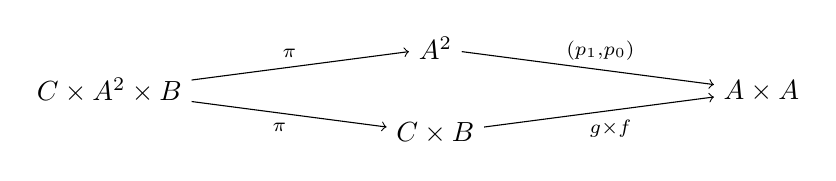
\begin{tikzpicture}[x=1.9em,y=1.4em]
  \node (L) at (0,0) {$C\times A^{2}\times B$};
  \node (T) at (6.2,1.1) {$A^{2}$};
  \node (B) at (6.2,-1.1) {$C\times B$};
  \node (R) at (12.4,0) {$A\times A$};
  \draw[->] (L) -- node[above,pos=0.45]{$\scriptstyle\pi$} (T);
  \draw[->] (L) -- node[below,pos=0.45]{$\scriptstyle\pi$} (B);
  \draw[->] (T) -- node[above,pos=0.55]{$\scriptstyle(p_{1},p_{0})$} (R);
  \draw[->] (B) -- node[below,pos=0.55]{$\scriptstyle g\times f$} (R);
\end{tikzpicture}
\end{center}
它计算 \eqref{eq:comma-pullback} 的拉回。\trUniversalProperty{} \eqref{eq:weighted-universal-property}
提供了 $\mathcal{K}$ 中的诸\trFunctor{} $\qcor{\alpha}\colon X\to\mathrm{Hom}_{A}(f,g)$
与诸单纯\trNaturalTransformation{}之间的一个对应，其
数据由恰好拼入两个交换方块的三支竖直虚映射给出：
\begin{center}
\begin{tikzpicture}[x=1.8em,y=1.4em]
  \node (1l) at (0,1.5) {$\mathbb{1}$};
  \node (two) at (3.6,1.5) {$2$};
  \node (1r) at (7.2,1.5) {$\mathbb{1}$};
  \draw[right hook->] (0.55,1.5) -- node[above]{$\scriptstyle 1$} (3.05,1.5);
  \draw[right hook->] (6.65,1.5) -- node[above]{$\scriptstyle 0$} (4.15,1.5);
  \draw[->,dashed] (0,1.05) -- node[left]{$\scriptstyle c$} (0,0.5);
  \draw[->,dashed] (3.6,1.05) -- node[right]{$\scriptstyle\qcor{\alpha}$} (3.6,0.5);
  \draw[->,dashed] (7.2,1.05) -- node[right]{$\scriptstyle b$} (7.2,0.5);
  \node (FL) at (0,0) {$\Fun(X,C)$};
  \node (FM) at (3.6,0) {$\Fun(X,A)$};
  \node (FR) at (7.2,0) {$\Fun(X,B)$};
  \draw[->] (1.35,0) -- node[below]{$\scriptstyle g\circ-$} (2.75,0);
  \draw[->] (6.35,0) -- node[below]{$\scriptstyle f\circ-$} (4.95,0);
\end{tikzpicture}
\end{center}
\end{example}

\begin{example}[作为加权余／极限的 Kan 扩张]\label{exa:kan-extensions-weighted}
计算一支非富集\trFunctor{} $F\colon C\to E$ 沿 $K\colon C\to D$ 的逐点左或右
Kan 扩张在对象 $d\in D$ 处之值的通常余极限或极限公式，可以由\trWeightedColimit{}或%
\trWeightedLimit{}简洁地表达为
\[ \lan_{K}F(d)\coloneqq\wcolim_{D(K-,d)}F
   \qquad\text{以及}\qquad
   \ran_{K}F(d)\coloneqq\wlim_{D(d,K-)}F. \]
\end{example}

\cref{def:weighted-limit-colimit-constructive}的诸公式给出了保证\trWeightedLimit{}或%
\trWeightedColimit{}得以存在的若干判据。

\begin{corollary}\label{cor:cotensors-conical-imply-weighted}
一个容有余张量、并对一切小的非富集\trDiagram{}形状容有锥形极限的 $\mathcal{V}$-%
\trCategory，便容有一切小的\trWeightedLimit。对偶地，一个容有张量、并对一切小的非富集%
\trDiagram{}形状容有锥形余极限的 $\mathcal{V}$-\trCategory，便容有一切小的%
\trWeightedColimit。
\end{corollary}

\begin{definition}\label{def:v-complete-v-cocomplete}
一个 $\mathcal{V}$-\trCategory{}是 $\mathcal{V}$-\textbf{\trComplete}
（$\mathcal{V}$-complete），若它容有诸小的 $\mathcal{V}$-\trWeightedLimit；或者等价
地，由\cref{cor:cotensors-conical-imply-weighted}，若它容有 $\mathcal{V}$ 中诸
对象所作的余张量以及小的锥形极限。对偶地，一个 $\mathcal{V}$-\trCategory{}是
$\mathcal{V}$-\textbf{\trCocomplete}（$\mathcal{V}$-cocomplete），若它容有诸
小的 $\mathcal{V}$-\trWeightedColimit；或者等价地，由%
\cref{cor:cotensors-conical-imply-weighted}，若它容有 $\mathcal{V}$ 中诸对象所
作的张量以及小的锥形余极限。
\end{definition}

\begin{remark}[论富集完备性的证明]\label{rem:proving-enriched-completeness}
在实践中，人们常如此证明一个 $\mathcal{V}$-\trCategory{}是完备的：证明其底%
\trCategory{}是完备的，并且该 $\mathcal{V}$-\trCategory{}同时容有余张量与张量
——后者乃是\trWeightedColimit{}的一个实例。然后施加\cref{prop:tensors-cotensors-conical}以确立：诸非富集的%
\trLimit{}事实上是锥形极限。
\end{remark}

我们以\trWeightedLimit{}与\trWeightedColimit{}一般理论中的若干结果来结束本节。从它们定义性的%
\trUniversalProperty{}出发立即可验证：

\begin{lemma}[受限\trDiagram{}的\trWeightedLimit]\label{lem:weighted-limits-restricted-diagrams}
设 $K\colon\mathcal{A}\to\mathcal{B}$ 是一支 $\mathcal{V}$-\trFunctor，
$W\colon\mathcal{A}\to\mathcal{V}$ 是一个权，而 $F\colon\mathcal{B}\to\mathcal{C}$
与 $G\colon\mathcal{B}^{\mathrm{op}}\to\mathcal{C}$ 是两个\trDiagram。于是，
受限\trDiagram{}的 $W$-\trWeightedLimit{}或\trWeightedColimit，同构于原\trDiagram{}的
$\lan_{K}W$-\trWeightedLimit{}或\trWeightedColimit：
\[ \wlim^{\mathcal{A}}_{W}(F\circ K)\cong\wlim^{\mathcal{B}}_{\lan_{K}W}F
   \qquad\text{以及}\qquad
   \wcolim^{\mathcal{A}}_{W}(G\circ K)\cong\wcolim^{\mathcal{B}}_{\lan_{K}W}G. \]
\end{lemma}

\begin{proof}
\cref{ex:prove-restricted-weighted-limits}。
\end{proof}

回忆\cref{def:vadjunction}：一个富集\trAdjunction{}由一对 $\mathcal{V}$-%
\trFunctor{} $F\colon\mathcal{B}\to\mathcal{A}$ 与
$U\colon\mathcal{A}\to\mathcal{B}$ 连同一族在两个变量中都是 $\mathcal{V}$-自然的%
\trIsomorphism{} $\mathcal{A}(Fb,a)\cong\mathcal{B}(b,Ua)$ 构成。通常的
Yoneda 式论证经富集化而表明：

\begin{proposition}\label{prop:enriched-adjoints-preserve-weighted-limits}
富集右伴随保持\trWeightedLimit，而富集左伴随保持\trWeightedColimit。
\end{proposition}

\begin{proof}
\cref{ex:prove-adjoints-preserve-weighted}。
\end{proof}

\subsection*{练习}

\begin{exercise}\label{ex:weighted-limits-of-simplicial-set}
把富集之基 $\mathcal{V}$ 取为 $\mathcal{S}et$，试计算单纯集 $X$——把它视作
$\mathcal{S}et^{\boldsymbol{\Delta}^{\mathrm{op}}}$ 中的一个\trDiagram{}——的
下列诸\trWeightedLimit，其权分别取：
\begin{enumerate}[label=(\roman*)]
\item 标准 $n$-\trSimplex{}
  $\Delta[n]\in\mathcal{S}et^{\boldsymbol{\Delta}^{\mathrm{op}}}$；
\item $n$-\trSimplex{}的\textbf{\trSpine}——把从 $i$ 到 $i+1$ 的那 $n$ 条边
  粘合为一条可复合的路径所得的 $\Delta[n]$ 的单纯子集；
\item $n$-\trSimplex{}边缘
  $\partial\Delta[n]\in\mathcal{S}et^{\boldsymbol{\Delta}^{\mathrm{op}}}$。
  \footnote{以 $\partial\Delta[n]$ 加权的单纯对象之\trLimit{}称为第 $n$ 个%
  \textbf{匹配对象}（$n$th-matching object）（见定义 C.4.14）。}
\end{enumerate}
\end{exercise}

\begin{exercise}\label{ex:prove-restricted-weighted-limits}
证明\cref{lem:weighted-limits-restricted-diagrams}。
\end{exercise}

\begin{exercise}\label{ex:prove-adjoints-preserve-weighted}
证明\cref{prop:enriched-adjoints-preserve-weighted-limits}。
\end{exercise}

\begin{exercise}\label{ex:enriched-profunctor-weights}
\begin{enumerate}[label=(\roman*)]
\item 把\trWeightedLimit{}与\trWeightedColimit{}的定义扩展到容许权 $W$ 为一个\textbf{富集泛函子}
  （enriched profunctor）——意即一支 $\mathcal{V}$-\trFunctor{}
  $W\colon\mathcal{B}^{\mathrm{op}}\times\mathcal{A}\to\mathcal{V}$，其中
  $\mathcal{A}$ 与 $\mathcal{B}$ 是小 $\mathcal{V}$-\trCategory{}——并使得%
  \trWeightedLimit{}与\trWeightedColimit{}\trFunctor{}具有如下形式：
  \[ (\mathcal{V}^{\mathcal{B}^{\mathrm{op}}\times\mathcal{A}})^{\mathrm{op}}
       \times\mathcal{C}^{\mathcal{A}}
       \xrightarrow{\ \wlim_{--}\ }\mathcal{C}^{\mathcal{B}}
     \qquad\text{以及}\qquad
     \mathcal{V}^{\mathcal{B}^{\mathrm{op}}\times\mathcal{A}}
       \times\mathcal{C}^{\mathcal{B}}
       \xrightarrow{\ \wcolim_{--}\ }\mathcal{C}^{\mathcal{A}} \]
\item 证明 (i) 中的\trWeightedLimit{}与\trWeightedColimit{}二函子构成一个双变量伴随的三分之二，
  其带有一个 $\mathcal{V}$-自然\trIsomorphism
\[ \mathcal{C}^{\mathcal{A}}\bigl(\wcolim_{W}G,F\bigr)
   \cong\mathcal{C}^{\mathcal{B}}\bigl(G,\wlim_{W}F\bigr) \]
  对 $W\in\mathcal{V}^{\mathcal{B}^{\mathrm{op}}\times\mathcal{A}}$、
  $F\in\mathcal{C}^{\mathcal{A}}$ 与 $G\in\mathcal{C}^{\mathcal{B}}$。
\item (ii) 的双变量伴随的第三个二函子是什么？
\end{enumerate}
\end{exercise}

